\documentclass{beamer}
\mode<presentation>{\usetheme{Warsaw}}

\usefonttheme{professionalfonts} % using non standard fonts for beamer
\usefonttheme{serif} % default family is serif
\usepackage{fontspec}
\setmainfont{Liberation Serif}
\usepackage{datetime}
\usepackage{amsfonts}
\usepackage{amssymb}
\usepackage{amsmath}
\usepackage{amsthm}
\usepackage{graphicx}
\usepackage{graphics}
\usepackage{subfigure}
\usepackage{wrapfig}
\usepackage{tikz}
\graphicspath{{figures/}}
\title{Boltzmann equation \& transport properties}
\author{MR Torkamani \& M Afkani}
\institute{Kharazmi university}
\newdateformat{monthyeardate}{%
  \monthname[\THEMONTH], \THEYEAR}
\date{\monthyeardate\today}

\begin{document}
\begin{frame}
\titlepage
\end{frame}
%%%%%%%%%%%%%
\begin{frame}[allowframebreaks]{Outline}
  \tableofcontents[sections={1-2}]
    \framebreak
  \tableofcontents[sections={3-5}]
\end{frame}
%%%%%%%%%%%%%
\begin{frame}
\frametitle{Introduction}
\begin{itemize}
\item The carriers in a metal can be affected by external fields and temperature gradians.
\pause
\item We want to calculate ordinary transport properties when constant fields are applied.
\pause
\item Simplest approach to do this porblem is to set up the transport equation or Boltzmann equation.
\end{itemize}
\end{frame}
%%%%%%%%%%%%%
\section{Boltzmann equation}
\subsection{What is $f (\vec{r},\vec{k},t)$}
\begin{frame}
\frametitle{What is $f (\vec{r},\vec{k},t)$}
\begin{itemize}
\item $f (\vec{r},\vec{k},t)$: local concentration of carrier in the state $k$ in the neighburhood of the point $r$ in space.
\pause
\item Boltzmann's equation study $f (\vec{r},\vec{k},t)$ changes over time.
\pause
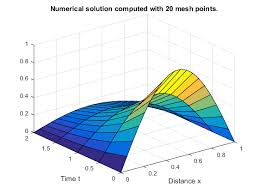
\includegraphics[scale=.7]{boltzmann}
\end{itemize}
\end{frame}
%%%%%%%%%%%%%
%\begin{frame}
%\frametitle{What is $f (r)$}
%\begin{align*}
%\dfrac{df}{dt} = \dfrac{\partial f}{\partial t} \dfrac{dt}{dt} + \dfrac{\partial f}{\partial r} \dfrac{dr}{dt} + \dfrac{\partial f}{\partial k} \dfrac{dk}{dt} 
%\end{align*}
%\begin{align*}
%\dfrac{df}{dt} = \dfrac{\partial f}{\partial t} \Big|_{scatt} + \dfrac{\partial f}{\partial t} \Big|_{diff} + \dfrac{\partial f}{\partial t}  \Big|_{field} 
%\end{align*}
%\end{frame}
%%%%%%%%%%%%%
\subsection{Changing $f (\vec{r},\vec{k},t)$ with time}
\begin{frame}
\frametitle{Diffusion}
\begin{columns}
\column{0.5\textwidth}
\pause
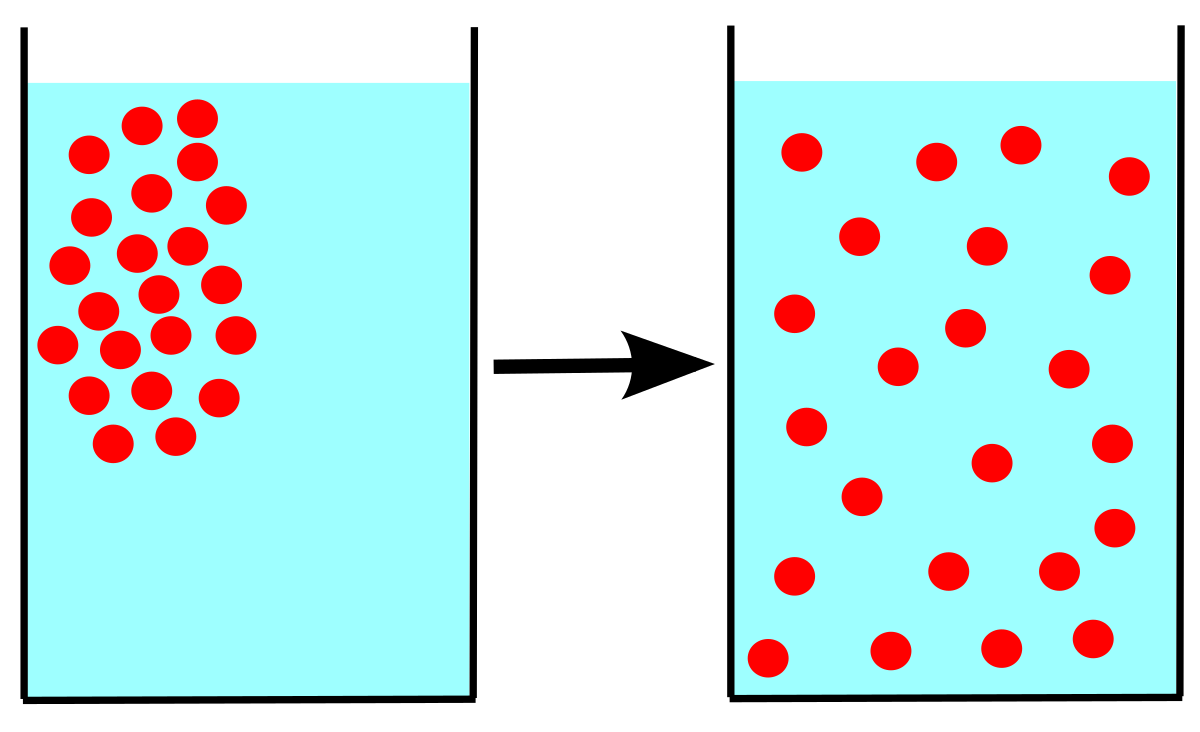
\includegraphics[scale=.1]{diffusion}
\column{0.5\textwidth}
\begin{itemize}
\pause
\item $\vec{v_k}$ is the velocity of a carrier in state $k$ .
\end{itemize}
\pause
\begin{align*}
f (\vec{r},\vec{k},\Delta t) &= f (\vec{r}-\vec{v_k} \Delta t,k ,0) 
\end{align*}
\pause
\begin{align*}
\dfrac{\partial f}{\partial t} &= \dfrac{f (\vec{r},\vec{k},\Delta t) - f (\vec{r},\vec{k},0)}{\Delta t}  
\end{align*}
\pause
\begin{align*}
\dfrac{\partial f}{\partial t}\big| _{diff} &= -\vec{v_k} .\nabla f
\end{align*}
\end{columns}
\end{frame}
%%%%%%%%%%%%%
\begin{frame}
\frametitle{Electromagnetic field}
\begin{columns}
\column{.4\textwidth}
\pause
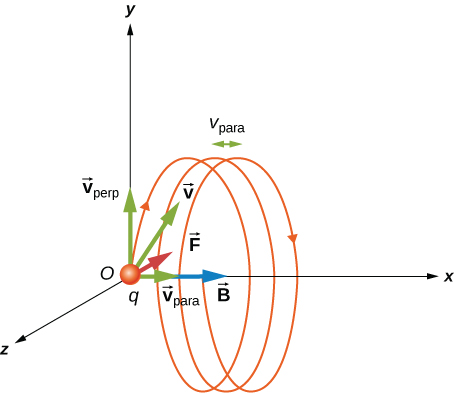
\includegraphics[scale=.4]{electromagnetic}
\column{.6\textwidth}
\begin{itemize}
\pause
\item external fields will change the k-vector of each carrier.
\end{itemize}
\pause
\begin{align*}
\vec{\dot{k}} = \dfrac{e}{\hslash} (\vec{E}+\dfrac{1}{c} \vec{v_k}\times \vec{H})
\end{align*}
\pause
\begin{itemize}
\item thus : $f (\vec{r},\vec{k},\Delta t) = f (\vec{r},\vec{k}-\vec{\dot{k}}\Delta t,0)$ in $k$-space.
\end{itemize}
\pause
\begin{align*}
\dfrac{\partial f}{\partial t}\Big| _{field} &= -\dfrac{e}{\hslash} (\vec{E}+\dfrac{1}{c} \vec{v_k}\times \vec{H}) .\nabla_k f
\end{align*}
\end{columns}
\end{frame}
%%%%%%%%%%%%%
\begin{frame}
\frametitle{Scattering}
\begin{columns}
\column{.5\textwidth}
\pause
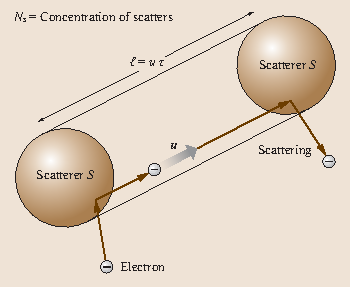
\includegraphics[scale=.4]{scattering}
\column{.5\textwidth}
\begin{itemize}
\pause
\item the effect of scattering is more complicated.
\end{itemize}
\pause
\begin{align*}
&\dfrac{\partial f}{\partial t}\Big| _{scatt} = \\& \int \big\{ f^\prime (1-f) - &f(1-f^\prime) \big\} Q(k,k^\prime) dk^\prime 
\end{align*}
\end{columns}
\end{frame}
%%%%%%%%%%%%%
\subsection{Boltzmann equation}
\begin{frame}
\frametitle{Boltzmann equation}
The Boltzmann transport equation is a statement that in the steady state, there is no net
change in the distribution function $f (\vec{r}, \vec{k}, t)$ which determines the probability of finding an electron at position $\vec{r}$ , crystal momentum $\vec{k}$ and time t. Therefore we get a zero sum for the changes in $f (\vec{r}, \vec{k}, t)$ due to the 3 processes of diffusion, the effect of forces and fields, and collisions
\pause
\begin{theorem}{Boltzman equation}
\begin{equation*}
\dfrac{df}{dt}=\dfrac{\partial f}{\partial t}\big| _{diff} +\dfrac{\partial f}{\partial t}\big| _{field}+ \dfrac{\partial f}{\partial t}\big| _{scatt} = 0
\end{equation*}
\end{theorem}
\end{frame}
%%%%%%%%%%%%%
\subsection{What is $g (\vec{r},\vec{k},t)$}
\begin{frame}
\frametitle{What is $g (\vec{r},\vec{k},t)$}
\pause
\begin{itemize}
\item $f^0$ : equilibrium distribution
\end{itemize}
\pause
\begin{align*}
f^0 = \dfrac{1}{e^{(\varepsilon_k -\zeta)/KT}} = f^0 (\varepsilon_k)
\end{align*}
\pause
\begin{align*}
g (\vec{r},\vec{k},t) = f (\vec{r},\vec{k},t) - f^0
\end{align*}
\pause
\begin{figure}[h]
\centering
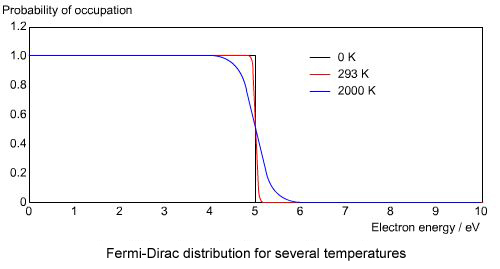
\includegraphics[scale=.3]{fermiDirac}
\end{figure}
\end{frame}
%%%%%%%%%%%%%
\subsection{Velocity of an electron!}
\begin{frame}
\frametitle{Velocity of an electron!}
\begin{itemize}
\pause
\item the velocity of an electron in the state $|k>$ is just the gradient of $\varepsilon (k)$ in k-space.
\end{itemize}
\pause
\begin{align*}
\vec{v} = \dfrac{1}{\hslash} \nabla _k \varepsilon (k)
\end{align*}
\pause
for free electron 
\begin{align*}
\varepsilon (k) = \dfrac{\hslash^2 k^2}{2m}
\end{align*}
\begin{align*}
\vec{v} = \dfrac{\hslash \vec{k}}{m} = \dfrac{\vec{p}}{m}
\end{align*}
\end{frame}
%%%%%%%%%%%%%
\begin{frame}
\frametitle{Boltzmann equation}
\begin{align*}
(- \dfrac{\partial f^0}{\partial \varepsilon}) \vec{v_k} . (-\dfrac{\varepsilon (k) - \zeta}{T}) \nabla T + e (\vec{E} - 1/c \nabla \zeta) \\
= \dfrac{\partial f}{\partial t} \big| _{scatt} + \vec{v_k}.\dfrac{\partial g}{\partial r} + \dfrac{e}{\hslash c} (\vec{v_k} \times \vec{H}) . \dfrac{\partial g}{\partial k}
\end{align*}
\end{frame}
%%%%%%%%%%%%%
\section{Electrical conductivity}
\subsection{Boltzmann equation}
\begin{frame}
\frametitle{Boltzmann equation}
suppose we have only an electic field $\vec{E}$
\pause
\begin{align*}
(- \dfrac{\partial f^0}{\partial \varepsilon}) \vec{v_k} . e \vec{E} = -\dfrac{\partial f}{\partial t} \big| _{scatt}
\end{align*}
\pause
\begin{align*}
-\dfrac{\partial f}{\partial t} \big| _{scatt} = \dfrac{g}{\tau} \quad  \text{assumption}
\end{align*}
\pause
\begin{align*}
g(t) = g(0)e^{- \dfrac{t}{\tau}}
\end{align*}
\pause
\begin{align*}
\boxed{g = (- \dfrac{\partial f^0}{\partial \varepsilon}) \vec{v_k} . e \tau \vec{E}} 
\end{align*}
\end{frame}
%%%%%%%%%%%%%
\subsection{Current density}
\begin{frame}
\frametitle{Current density}
\pause
\begin{align*}
\vec{J} = 2 \int e v_k f (\vec{r},\vec{k},t) d^3k
\end{align*}
\pause
\begin{align*}
\vec{J} = 2 \int e \vec{v_k} g (r,k,t) dk \quad (\text{since} \int \vec{v_k} f^0 dk \equiv 0) 
\end{align*}
\pause
\begin{align*}
\vec{J} = \dfrac{1}{4 \pi ^3} \int \int e^2 \tau \vec{v_k}.\vec{E} (- \dfrac{\partial f^0}{\partial \varepsilon}) \dfrac{ds}{\hslash v_k}d\varepsilon 
\end{align*}
\pause
\begin{align*}
\vec{J} = \dfrac{1}{4 \pi ^3} \dfrac{e^2 \tau}{\hslash} \int \dfrac{\vec{v_k}\vec{v_k}}{v_k}ds_f .\vec{E}
\end{align*}
\end{frame}
%%%%%%%%%%%%%
\subsection{Conducting scalar I}
\begin{frame}
\frametitle{conducting scalar}
\begin{itemize}
\item we usually deal with crystals having cubic symmetry in which case the conductivity tensor reduce to  an scalar.
\pause
\item thinking of the case where $\vec{E}$ and $\vec{J}$ both in x-direction.
\end{itemize}
\pause
\begin{align*}
(\vec{v_k}\vec{v_k}.\vec{E})_x = v_x^2 E = \dfrac{1}{3} v^2 E
\end{align*}
\pause
\begin{align*}
\sigma = \dfrac{1}{4 \pi ^3} \dfrac{e^2}{3 \hslash} \int \Lambda ds_f  \qquad \Lambda = \tau v
\end{align*}
\end{frame}
%%%%%%%%%%%%%
\subsection{Conducting scalar II}
\begin{frame}
\frametitle{conducting scalar}
\pause
\begin{align*}
g = f - f^0 (k) = -\dfrac{\partial f^0}{\partial \varepsilon} \dfrac{\partial \varepsilon}{\partial k} . \dfrac{e\tau}{\hslash} \vec{E}
\end{align*}
\pause
\begin{align*}
f = f^0 (k-\dfrac{e\tau}{\hslash} \vec{E}) \qquad \text{in k-space}
\end{align*}
\pause
\begin{align*}
f = f^0 (\varepsilon_k - e\tau \vec{v_k}.\vec{E}) \qquad \delta \varepsilon_k =e\tau \vec{v_k}.\vec{E} 
\end{align*}
\pause
\begin{align*}
\delta \vec{v} \dfrac{\partial \varepsilon}{\partial v} =e\tau \vec{v_k}.\vec{E} \Rightarrow \delta \vec{v} =\dfrac{ev\tau}{mv} \vec{E} 
\end{align*}
\pause
\begin{align*}
\vec{J}= ne \delta \vec{v} = \dfrac{ne^2\tau}{m}\vec{E}
\end{align*}
\end{frame}
%%%%%%%%%%%%%
\section{General Transport equation}
\subsection{Boltzmann equation}
\begin{frame}
\frametitle{Boltzmann equation}
suppose now that we have a temperature gradient in the specimen as well as an electric field. ignoring size and shape effects.
\pause
\begin{align*}
(- \dfrac{\partial f^0}{\partial \varepsilon}) \vec{v_k} . (-\dfrac{\varepsilon (k) - \zeta}{T}) \nabla T + e (\vec{E} - 1/c \nabla \zeta) = \dfrac{\partial f}{\partial t} \big| _{scatt}
\end{align*}
\pause
\begin{align*}
\vec{J} &= \dfrac{1}{4\pi^3} \dfrac{e^2 \tau}{\hslash} \int \int \vec{v_k}\vec{v_k} (- \dfrac{\partial f^0}{\partial \varepsilon}) \dfrac{ds}{v_k} d\varepsilon .(\vec{E} - \dfrac{1}{e} \nabla \zeta)\\
&+ \dfrac{1}{4\pi^3} \dfrac{e^2 \tau}{\hslash} \int \int \vec{v_k}\vec{v_k} (\dfrac{\varepsilon - \zeta}{T})(- \dfrac{\partial f^0}{\partial \varepsilon}) \dfrac{ds}{v_k} d\varepsilon .(-\nabla T)
\end{align*}
\end{frame}
%%%%%%%%%%%%%
\subsection{Heat}
\begin{frame}
\frametitle{Heat}
\begin{itemize}
\item heat $=$ internal energy $-$ free energy
\pause
\item the total flux of heat (per unit volume) is:
\end{itemize}
\begin{align*}
\vec{U} = 2 \int  (\varepsilon - \zeta)f(\vec{r},\vec{k},t) v_k d^3k
\end{align*}
\end{frame}
%%%%%%%%%%%%%
\subsection{General Transport equation}
\begin{frame}
\frametitle{General Transport equation}
\begin{align*}
\vec{J} &= e^2 \overleftrightarrow{K_0}.\vec{E} +\dfrac{e}{T} \overleftrightarrow{K_1} . (- \nabla T)\\
\vec{U} &= e \overleftrightarrow{K_1}.\vec{E} +\dfrac{1}{T} \overleftrightarrow{K_2} . (- \nabla T)
\end{align*}
\pause
\begin{align*}
\overleftrightarrow{k_n} \equiv \dfrac{1}{4 \pi ^3} \dfrac{\tau}{\hslash} \int \int \vec{v} \vec{v} (\varepsilon - \zeta)^n (- \dfrac{\partial f^0}{\partial \varepsilon}) \dfrac{ds}{v} d\varepsilon
\end{align*}
\pause
\begin{align*}
\overleftrightarrow{K_0} &= \dfrac{\tau}{4\pi^3 \hslash} \int \vec{v}\vec{v} \dfrac{ds_f}{v} \quad
\overleftrightarrow{K_2} = \dfrac{1}{3}\pi^2 (kT)^2 K_0 (\zeta)\\
\overleftrightarrow{K_1} &= \dfrac{1}{3}\pi^2 (kT)^2 \dfrac{\partial}{\partial \varepsilon} K_0 (\varepsilon) \big| _{\varepsilon = \zeta} 
\end{align*}
\end{frame}
%%%%%%%%%%%%%
\subsection{Thermal conductivity}
\begin{frame}
\frametitle{Thermal conductivity}
\pause
\begin{align*}
\vec{E} = \dfrac{1}{e^2} K^{-1}_{0} K_1 \dfrac{e}{T} (-\nabla T)
\end{align*}
\pause
\begin{align*}
\vec{U} &= \dfrac{1}{T} K_1 K^{-1}_{0} K_1 . \nabla T - \dfrac{1}{T} K_2 . \nabla T \\
\vec{U} &= \dfrac{1}{T} (-K_1 K^{-1}_{0} K_1 + K_2).(-\nabla T) \\
\vec{U} &= \kappa .(-\nabla T)
\end{align*}
\pause
But for metal, we can ignore the $K_1 K^{-1}_{0} K_1$ 
\begin{align*}
\kappa = \dfrac{1}{T} K_2
\end{align*}
\end{frame}
%%%%%%%%%%%%%
\begin{frame}
\frametitle{Wiedemann-Franz law}
\pause
the coefficient of $\vec{E}$ in $\vec{J}$ equation is $\sigma$
\begin{align*}
\sigma = e^2 K_0
\end{align*}
\pause
\begin{align*}
K_2 &= \dfrac{1}{3}\pi^2 (kT)^2 K_0 (\zeta)
\end{align*}
\pause
\begin{align*}
\boxed{\kappa = \dfrac{\pi^2}{3} \dfrac{k^2}{e^2} T \sigma}
\end{align*}
\end{frame}
%%%%%%%%%%%%%
\subsection{Compair Electrical and Thermal conduction}
\begin{frame}
\frametitle{Compair Electrical and Thermal conduction}
\begin{table}
\centering
\begin{tabular}{|c|c|}
\hline
electircal conduction & thermal conduction \\
\hline
each electorn carries its & each electron carries thermal\\
charge $e$,&  energy $kT$ its acted \\
and is acted on by & by a thermal force $k \nabla T$ \\
the field $e\vec{E}$ & the heat current per unit  \\
the current per unit field &  thermal gradient \\
is proportional to $e^2$ & is proportional to $k^2 T$\\
\hline  
\end{tabular}
\end{table}
the ratio of these two transport coefficients $= \dfrac{k^2 T}{e^2}$
\end{frame}
%%%%%%%%%%%%%
\section{Thermo-electric effects}
\subsection{Seebeck effect}
\begin{frame}
\frametitle{Seebeck effect}
\pause
in open circuit with thermal gradient we have:
\begin{align*}
\vec{E} = \dfrac{1}{e T} K^{-1}_{0} K_1 (\nabla T) = Q \nabla T
\end{align*}
\pause
\begin{figure}[h]
\centering
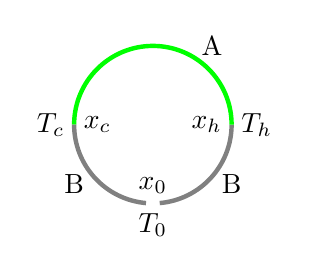
\begin{tikzpicture}[scale = .5]
\draw [gray,ultra thick] (6,0) arc [radius=2, start angle=0, end angle= -85];
\draw [green,ultra thick] (6,0) arc [radius=2, start angle=0, end angle= 180];
\draw [gray,ultra thick] (2,0) arc [radius=2, start angle=180, end angle= 265];
\node [left] at (2,0) {$T_c$};
\node [right] at (2,0) {$x_c$};
\node [right] at (6,0) {$T_h$};
\node [left] at (6,0) {$x_h$};
\node [above] at (5.5,1.5) {A};
\node [above] at (4,-2) {$x_0$};
\node [below] at (4,-2) {$T_0$};
\node at (2,-1.5) {B};
\node at (6,-1.5) {B};
\end{tikzpicture}
\end{figure}
\pause
\begin{align*}
V = \int_{x_0}^{x_c} E_B dx +\int_{x_c}^{x_h}E_A dx +\int_{x_h}^{x_0}E_B dx = \int_{T_c}^{T_h} (Q_A - Q_B) dT 
\end{align*}
\end{frame}
%%%%%%%%%%%%%
\subsection{Peltier effect}
\begin{frame}
\frametitle{Peltier effect}
suppose we keep $\nabla T = 0$ round the same circuit
\begin{align*}
\vec{U} = eK_1 \vec{E} \qquad \vec{J} = e^2K_0 \vec{E} \\
\vec{U} = \dfrac{1}{e} K_{0}^{-1}K_1 \vec{J} = \Pi \vec{J}
\end{align*} 
\pause
\begin{figure}[h]
\centering
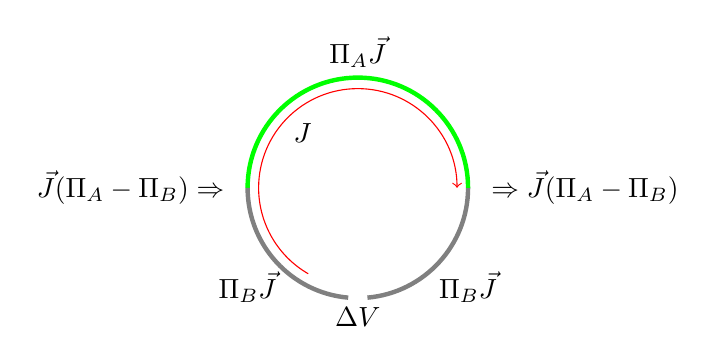
\begin{tikzpicture}[scale = .7]
\draw [gray,ultra thick] (6,0) arc [radius=2, start angle=0, end angle= -85];
\draw [green,ultra thick] (6,0) arc [radius=2, start angle=0, end angle= 180];
\draw [<-,red] (5.8,0) arc [radius=1.8, start angle=0, end angle= 240];
\draw [gray,ultra thick] (2,0) arc [radius=2, start angle=180, end angle= 265];
\node [right] at (-2,0) {$\vec{J} (\Pi_A -\Pi_B) \Rightarrow$};
\node [left] at (10,0) {$\Rightarrow \vec{J} (\Pi_A -\Pi_B)$};
\node [above] at (4,2) {$\Pi_A \vec{J}$};
\node at (2,-1.8) {$\Pi_B \vec{J}$};
\node at (6,-1.8) {$\Pi_B \vec{J}$};
\node [below] at (4,-2) {$\Delta V$};
\node at (3,1) {$J$};
\end{tikzpicture}
\end{figure}
\end{frame}
%%%%%%%%%%%%%
\section{references}
\begin{frame}{references}
\begin{itemize}
\item Ziman, Principles of the Theory of Solids, Cambridge Univ. Press, 1972, Chapter 7
\item M. S. Dresselhaus, Transport Properties of Solids,MIT Univ. press, 2001, Chapters 4 and 5
\end{itemize}

\end{frame}
\end{document}
